% Vista preliminar del código fuente

%% LyX 2.0.0 created this file.  For more info, see http://www.lyx.org/.
%% Do not edit unless you really know what you are doing.
\documentclass[english]{article}
\usepackage[T1]{fontenc}
\usepackage[latin9]{inputenc}
\usepackage{float}
\usepackage{graphicx}

\makeatletter

%%%%%%%%%%%%%%%%%%%%%%%%%%%%%% LyX specific LaTeX commands.
%% Because html converters don't know tabularnewline
\providecommand{\tabularnewline}{\\}

%%%%%%%%%%%%%%%%%%%%%%%%%%%%%% Textclass specific LaTeX commands.
\newenvironment{lyxcode}
{\par\begin{list}{}{
\setlength{\rightmargin}{\leftmargin}
\setlength{\listparindent}{0pt}% needed for AMS classes
\raggedright
\setlength{\itemsep}{0pt}
\setlength{\parsep}{0pt}
\normalfont\ttfamily}%
 \item[]}
{\end{list}}

\makeatother

\usepackage{babel}
\begin{document}

\title{Aprendizaje Automático - Trabajo Práctico 5}


\author{Gonzalo Castiglione - $49138$}

\maketitle

\paragraph*{Objetivo: Aprender a tomar decisiones basadas en un árbol de decisión}


\section{Aprendizaje de árboles de decisiones}
\begin{enumerate}
\item La $entrop\acute{\imath}a$ para un conjunto de $ejemplos$ $S$ esta
dada por la fórmula
\[
E(S)=\sum_{i\epsilon C}-p_{i}log_{2}p_{i}
\]



En donde $C$ es el conjunto de clases a las quepueden perteneces
dichos ejemplos y $p_{i}$ es la probabilidad de que un ejemplo dado
pertenezca a la clase $i-esima$.
\begin{enumerate}
\item Sea el siguiente conjunto de entrenamiento:


\begin{center}
\begin{tabular}{|c|c|c|c|}
\hline 
Instancia & $a_{1}$ & $a_{2}$ & Clasificacion\tabularnewline
\hline 
\hline 
1 & T & T & +\tabularnewline
\hline 
2 & T & T & +\tabularnewline
\hline 
3 & T & F & -\tabularnewline
\hline 
4 & F & F & +\tabularnewline
\hline 
5 & F & T & -\tabularnewline
\hline 
6 & F & T & -\tabularnewline
\hline 
\end{tabular}
\par\end{center}


$p_{-}=p_{+}=0.5=p$


Dado que los patrones estan divididos exactamente a la mitad, es de
esperarse que el valor de la entropía sea maximo, es decir, 1.


$E(S)=-p_{+}log_{2}p_{+}-p_{-}log_{2}p_{-}=-2plog_{2}p=1$

\item En base a la entropia, se define la $ganancia$ $de$ $informaci\acute{o}n$
como la disminución de la entropia que se produce al dividir un conjunto
S de ejemplos según valores $v_{i}$ de un atributo $A$. Es decir:
\[
G(S,A)=E(S)-\sum_{v_{i}\epsilon V}\frac{|S_{v_{i}}|}{|S|}E(S_{v_{i}})
\]



donde $V$ es el conjunto de valores que puede tomar el atributo $A$,
y $S_{v_{i}}$, es el subconjunto de ejemplos de $S$ cuyo atributo
$A$ tiene el valores $v_{i}$. 


$G(S,a_{2})=1-\frac{4}{6}*1-\frac{2}{6}*1=0$

\end{enumerate}
\item ELIMINACIÓN- DE-CANDIDATOS Vs ID3

\begin{enumerate}
\item Arbol creado por el algoritmo:


\begin{figure}[H]
\centering{}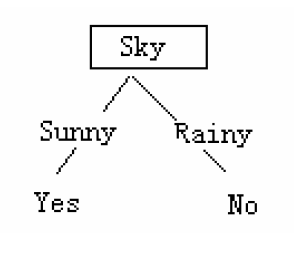
\includegraphics[scale=0.5]{2_ArbolDecis}\caption{Árbol de decisión generado a partir de la tabla dada}
\end{figure}


\item El espacio de versiones contiene todas las hipótesis consitentes con
los ejemplos de entrenamiento, mientras que el árbol de decisión aprendido
es una de las hipótesis consistentes con los ejemplos de entrenamiento. 
\item Resolución

\begin{enumerate}
\item Primero 


Entropia(X) = -3/5{*}log2(3/5)-2/5{*}log2(2/5) = 0.971 


G(X, cielo) = 0.971-4/5{*}(-3/4log2 (3/4)-(1/4)log2(1/4))-1/5{*}0
= 0.322 


G(X, tempAire) = 0.971-4/5{*}(-3/4log2 (3/4)-(1/4)log2(1/4))-1/5{*}0
= 0.322 


G(X, humedad) = 0.971-3/5{*}(-2/3log2 (2/3)-(1/3)log2(1/3))-2/5{*}1
= 0.02 


G(X, viento) = 0.971-4/5{*}(-3/4log2 (3/4)-(1/4)log2(1/4))-1/5{*}0
= 0.322 


G(X, tempAgua) = 0.971-4/5{*}(-2/4log2 (2/4)-(2/4)log2(2/4))-1/5{*}0
= 0.171 


G(X, pronostico) = 0.971-3/5{*}(-2/3log2 (2/3)-(1/3)log2(1/3))-2/5{*}1
= 0.02 
\begin{itemize}
\item El algorimto elige \textquotedblleft{}cielo\textquotedblright{} como
el atributo de testeo para la raiz.
\end{itemize}
\item Segundo


Entropia(X) = -3/4{*}log2(3/4)-1/4{*}log2(1/4) = 0.8113 


G(X, tempAire) = 0 


G(X, humedad) = 0.3113 


G(X, viento) = 0.8113 


G(X, tempAgua) = 0.1226 


G(X, pronostico) = 0.1226
\begin{itemize}
\item El algorimto elige \textquotedblleft{}viento\textquotedblright{}.
\end{itemize}
\end{enumerate}

Version final del arbol de decisión creado


\begin{figure}[H]
\centering{}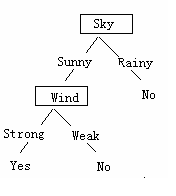
\includegraphics{3_ArbolDecis}\caption{Nuevo árbol creado a partir de la tabla original con el nuevo ejemplo}
\end{figure}


\end{enumerate}
\item Árbol generado para los lirios de $fisher$.


\begin{figure}[H]
\centering{}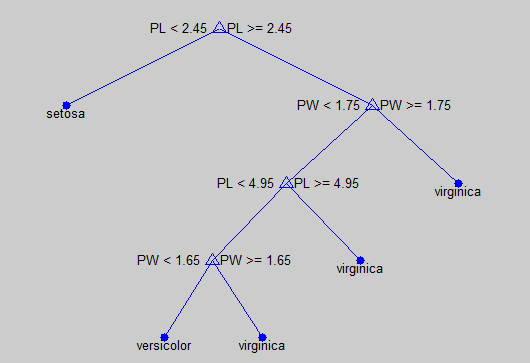
\includegraphics[scale=0.75]{fisheriris}\caption{Árbol creado a partir de las mediciones de los lirios de Fisher}
\end{figure}

\begin{lyxcode}
if~PL<2.45~then~node~2~

elseif~PL>=2.45~then~node~3~~\\
else~setosa
\begin{lyxcode}
class~=~setosa

if~PW<1.75~then~node~4~

elseif~PW>=1.75~then~node~5~

else~versicolor

if~PL<4.95~then~node~6~

elseif~PL>=4.95~then~node~7~

else~versicolor~5

~

class~=~virginica

if~PW<1.65~then~node~8~

elseif~PW>=1.65~then~node~9~

else~versicolor



class~=~virginica~

class~=~versicolor

class~=~virginica\end{lyxcode}
\end{lyxcode}
\end{enumerate}

\end{document}
